%%%%%%%%%%%%%%%%%%%%%%%%%%%%%%%%%%%%%%%%%%%%%%%%%%%%%%%%%%%%%%%%%%%%%%%%%%%%%%%%%%%%%%%%%%%%%%%%%%%%%%%%%%%%%%%%%%%%%%%%%%%%%%%%%%%%%%%%
% This is just a template to use when submitting manuscripts to Frontiers, it is not mandatory to use frontiers.cls nor frontiers.tex  %
%%%%%%%%%%%%%%%%%%%%%%%%%%%%%%%%%%%%%%%%%%%%%%%%%%%%%%%%%%%%%%%%%%%%%%%%%%%%%%%%%%%%%%%%%%%%%%%%%%%%%%%%%%%%%%%%%%%%%%%%%%%%%%%%%%%%%%%%

%\documentclass{frontiersENG} % for Engineering articles
\documentclass{frontiersSCNS} % for Science articles
%\documentclass{frontiersMED} % for Medicine articles

\usepackage{url}%,lineno}
\usepackage{floatrow}
\usepackage{subfig}
\usepackage{wrapfig}
\usepackage[font=small]{caption}

%\linenumbers
%\linespread{1.6} %doublespacing

% Leave a blank line between paragraphs in stead of using \\

\copyrightyear{}
\pubyear{}

\def\journal{Computational Neuroscience}%%% write here for which journal %%%
\def\DOI{}
\def\articleType{Research Article}
\def\keyFont{\fontsize{8}{11}\helveticabold }
\def\firstAuthorLast{Steele {et~al.}} %use et al only if is more than 1 author
\def\Authors{Sara Steele\,$^{1,*}$, Daniel Tranchina\,$^{2,3}$ and John Rinzel\,$^{1,2}$}
% Affiliations should be keyed to the author's name with superscript numbers and be listed as follows: Laboratory, Institute, Department, Organization, City, State abbreviation (USA, Canada, Australia), and Country (without detailed address information such as city zip codes or street names).
% If one of the authors has a change of address, list the new address below the correspondence details using a superscript symbol and use the same symbol to indicate the author in the author list.
\def\Address{$^{1}$Center for Neural Science, New York University, New York, NY, USA\\
$^{2}$Courant Institute for Mathematical Sciences, New York University, New York, NY, USA \\
$^{3}$Department of Biology, New York University, New York, NY, USA}
% The Corresponding Author should be marked with an asterisk
% Provide the exact contact address (this time including street name and city zip code) and email of the corresponding author
\def\corrAuthor{Sara Steele}
\def\corrAddress{Center for Neural Science, New York University, 4 Washington Pl, Room 809, 
New York, NY 10003, USA}
\def\corrEmail{steeles@cns.nyu.edu}

% \color{FrontiersColor} Is the color used in the Journal name, in the title, and the names of the sections


\begin{document}
\onecolumn
\firstpage{1}

\title[Alternating renewal process describes buildup]{From one to many (and back again): an alternating renewal process describes the buildup of perceptual segregation}
\author[\firstAuthorLast ]{\Authors}
\address{}
\correspondance{}
\extraAuth{}% If there are more than 1 additional author, comment this line and uncomment the next one
%\extraAuth{corresponding Author2 \\ Laboratory X2, Institute X2, Department X2, Organization X2, Street X2, City X2 , State XX2 (only USA, Canada and Australia), Zip Code2, X2 Country X2, email2@uni2.edu}
\topic{Research Topic}

\maketitle
\begin{abstract}

\section{}
For some ambiguous scenes, perceptual organization becomes more complex as a subject's presentation time increases, in that different stimulus features are gradually more likely to be grouped into different perceptual representations. In particular, the segregation of acoustic features into different streams takes time to build up. We compute the buildup function for a particular stimulus as the probability as a function of time that subjects report experiencing a split perceptual organization. Previous approaches to characterizing the buildup function relate the current perceptual state to some underlying mechanism of accumulation, of, for instance, adaptation. We present a statistical model from the theoretical framework of an alternating renewal process that produces buildup functions in the absence of any accumulative process. In this statistical model, the observer alternates between perceptual organizations, as in perceptual bistability, with dominance durations composed of random samples from independent density functions. Using this theory, we can describe the short term dynamics of buildup observed on short trials in terms of the long term statistics of percept durations for the two alternating perceptual organizations. This model performs well in describing buildup functions computed from pseudo-neuronal simulations of neural populations with competition architecture that undergo alternations. Depending on the parameters, these competition model simulations sometimes produce history dependence through accumulation of adaptation. Nonetheless, our switching model, which neglects history dependence from accumulative processes, is able to predict the buildup function. This indicates that accumulation is not a necessary feature to produce or to describe a buildup function. Rather, any model producing buildup will have an underlying alternating renewal process, the statistics of which are sufficient to account for buildup.

\tiny
 \keyFont{ \section{Keywords:} stream segregation; alternating renewal process; bistable perception; perceptual dynamics; perceptual organization } %All article types: you may provide up to 8 keywords; at least 5 are mandatory.
\end{abstract}


\section{Introduction}

For some stimuli in the auditory and visual modalities with ambiguous grouping cues, the probability of perceptual ``splitting" increases with time. One example of this is found in auditory stream segregation, using an ABA- stimulus (\cite{Noorden1975}). A and B refer to tones at different frequencies, and - represents a silent interval. Depending on the difference in frequency and presentation rate of the tones, listeners might be biased to hear grouped triplet patterns integrated into a galloping rhythm, or segregated streams of tones at separate frequencies (Figure \ref{fig:percepts_timecourse}). A number of studies using ambiguous ABA- tone sequences (\cite{Noorden1975}) have shown that perceptual splitting of sound events with different acoustic features increases over time (\cite{Bregman1978, Anstis1985,Cusack2004}). There is typically a period of time over which the probability of the segregated percept increases, starting from the initiation of a presentation (\cite{Bregman1978, Anstis1985}) or a switch in the focus of attention (\cite{Cusack2004}).  In addition, a similar phenomenon has been reported in the visual modality. When viewing ambiguous moving plaids constructed from two moving square wave gratings at intermediate speed and angle, observers have reported first experiencing coherent motion of a unified plaid pattern, even when, in the long term, their perception is biased towards transparent motion of the individual gratings in each of their component directions (\cite{Rubin2004}). The change in probability of observers reporting a split perceptual organization over time can be quantified as a buildup function. This can be stated quantitatively as $p_{z(t)=1|z(0)=0}$, where $z(t)=0$ indicates a grouped perceptual organization at time $t$ and $z(t)=1$ indicates a split perceptual organization. The psychophysical data show that such dynamically changing perceptual states are accompanied by reports of perceptual alternations (\cite{Deike2012}). %,Denham,buildup+alternations, some plaid buildups}. 
Because of the ambiguity of the stimuli, subjects report experiencing sudden switches between one perceptual state and the other (\cite{Pressnitzer2006, Hupe2012}) over long presentations, even after the buildup function has reached steady state.

\begin{figure}
	\centering
	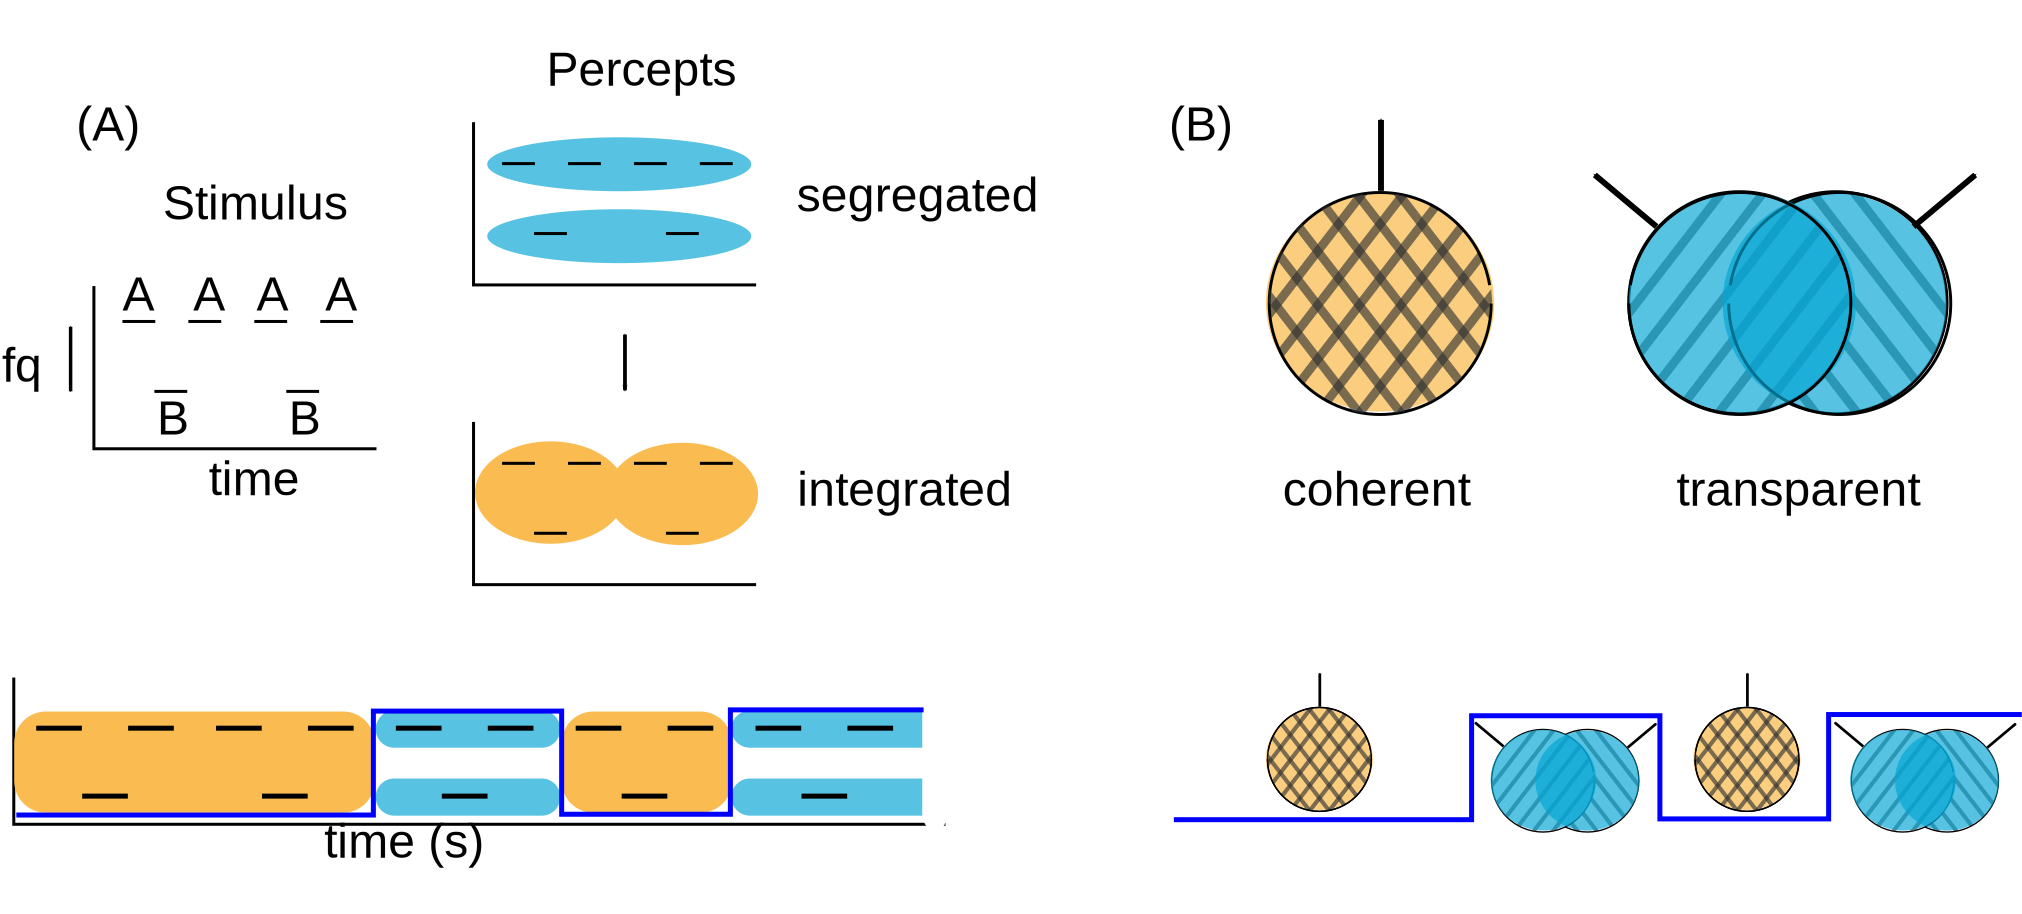
\includegraphics[scale=0.23]{../aba_plaid_stimulus-percepts}
	\caption{Examples of stimuli that can produce ambiguous grouping. \textbf{(a)} Van Noorden triplets with ambiguous stream segregation. Listeners report alternations between hearing integration (bottom, orange) and segregation (top, blue) of the component tone frequencies. \textbf{(b)} Moving gratings at certain angles can produce ambiguous motion. Observers report alternations between coherent and transparent motion of the component gratings.}
	\label{fig:percepts_timecourse}
\end{figure}

In the auditory domain, these perceptual dynamics have been a subject of great interest because they are thought to be a product of the same mechanisms that enable listeners to perceptually group components of an acoustic signal according to the sources that produced them, a process known as stream segregation. Many explanations of buildup appeal to proposed mechanisms of stream segregation. One theoretical explanation for the perceptual organizations observed with the ABA- stimuli is grouping by coactivation (for a review, see \cite{Carlyon2004}). Sound signals that excite the same population of neurons are grouped, whereas those which activate separate populations are perceived as coming from separate sources, that is, split. [elaborate?] Some theories (\cite{Micheyl2005,Pressnitzer2008,Bee2010}) propose that the buildup function reflects the accumulation of adaptation over seconds, or multi-second habituation, which leads to a decrease over time of activation by the other tone of auditory neurons tuned to each of the two tone frequencies.  %In general, the idea that buildup reflects a process by which the auditory system accumulates evidence is quite old (\cite{Bregman1990}). 

The accumulation-based account of the buildup function can quantitatively predict the switch from the grouped to the split percept; however, it is unable to explain why subjects undergo continued switches between perceptual organizations. We show that the buildup function can be described well by a model that uses the statistics of alternations, but no accumulation. The gradual increase in probability of a split percept over time could reflect the dynamics of an entirely random underlying alternating renewal process with a given initial state.

The long-term dynamics of perceptual bistability consist of alternations between mutually excusive percepts. The duration histogram of each percept is well-fit by a gamma density (\cite{Shpiro2009, Pressnitzer2006}). We believe that the short-term increase in probability of split percepts, observed when short trial perceptual timecourses are averaged, could reflect the dominance duration distributions observed over long trials. To examine this relationship we use the theoretical framework of an alternating renewal process (\cite{}). In this investigation we show that these distributions of percept durations, without consideration for history dependence between successive durations, can account for the experimentally observed perceptual dynamics for a stimulus with ambiguous grouping, as follows:

\begin{enumerate}
\item the perceptual state alternates back and forth between grouped and split
\item the durations for these perceptual epochs are random, independent and stationary
\item the initial percept on for a given presentation is always the grouped percept
\end{enumerate}

In addition, we use existing computational models of perceptual bistability to explore how different mechanisms of alternation affect the model's behavior with regard to the buildup function.

\section{Results}
\subsection*{Alternating renewal process}

The process of computing the buildup function empirically involves the averaging over many trials of the timecourse of a random binary state variable (see Figure \ref{fig:makingBUFs}a, blue lines). In our statistical model, the initial state (percept) is fixed, but the dwell time in this state is a random variable characterized by its probability density function. Subsequently the system switches randomly between two states, each of which has its own fixed duration distribution.

\floatsetup[figure]{style=plain,subcapbesideposition=top}
%\begin{wrapfigure}{R}{1\textwidth}
\begin{figure}	
	\centering
	
	  \sidesubfloat[]{\label{fig:a}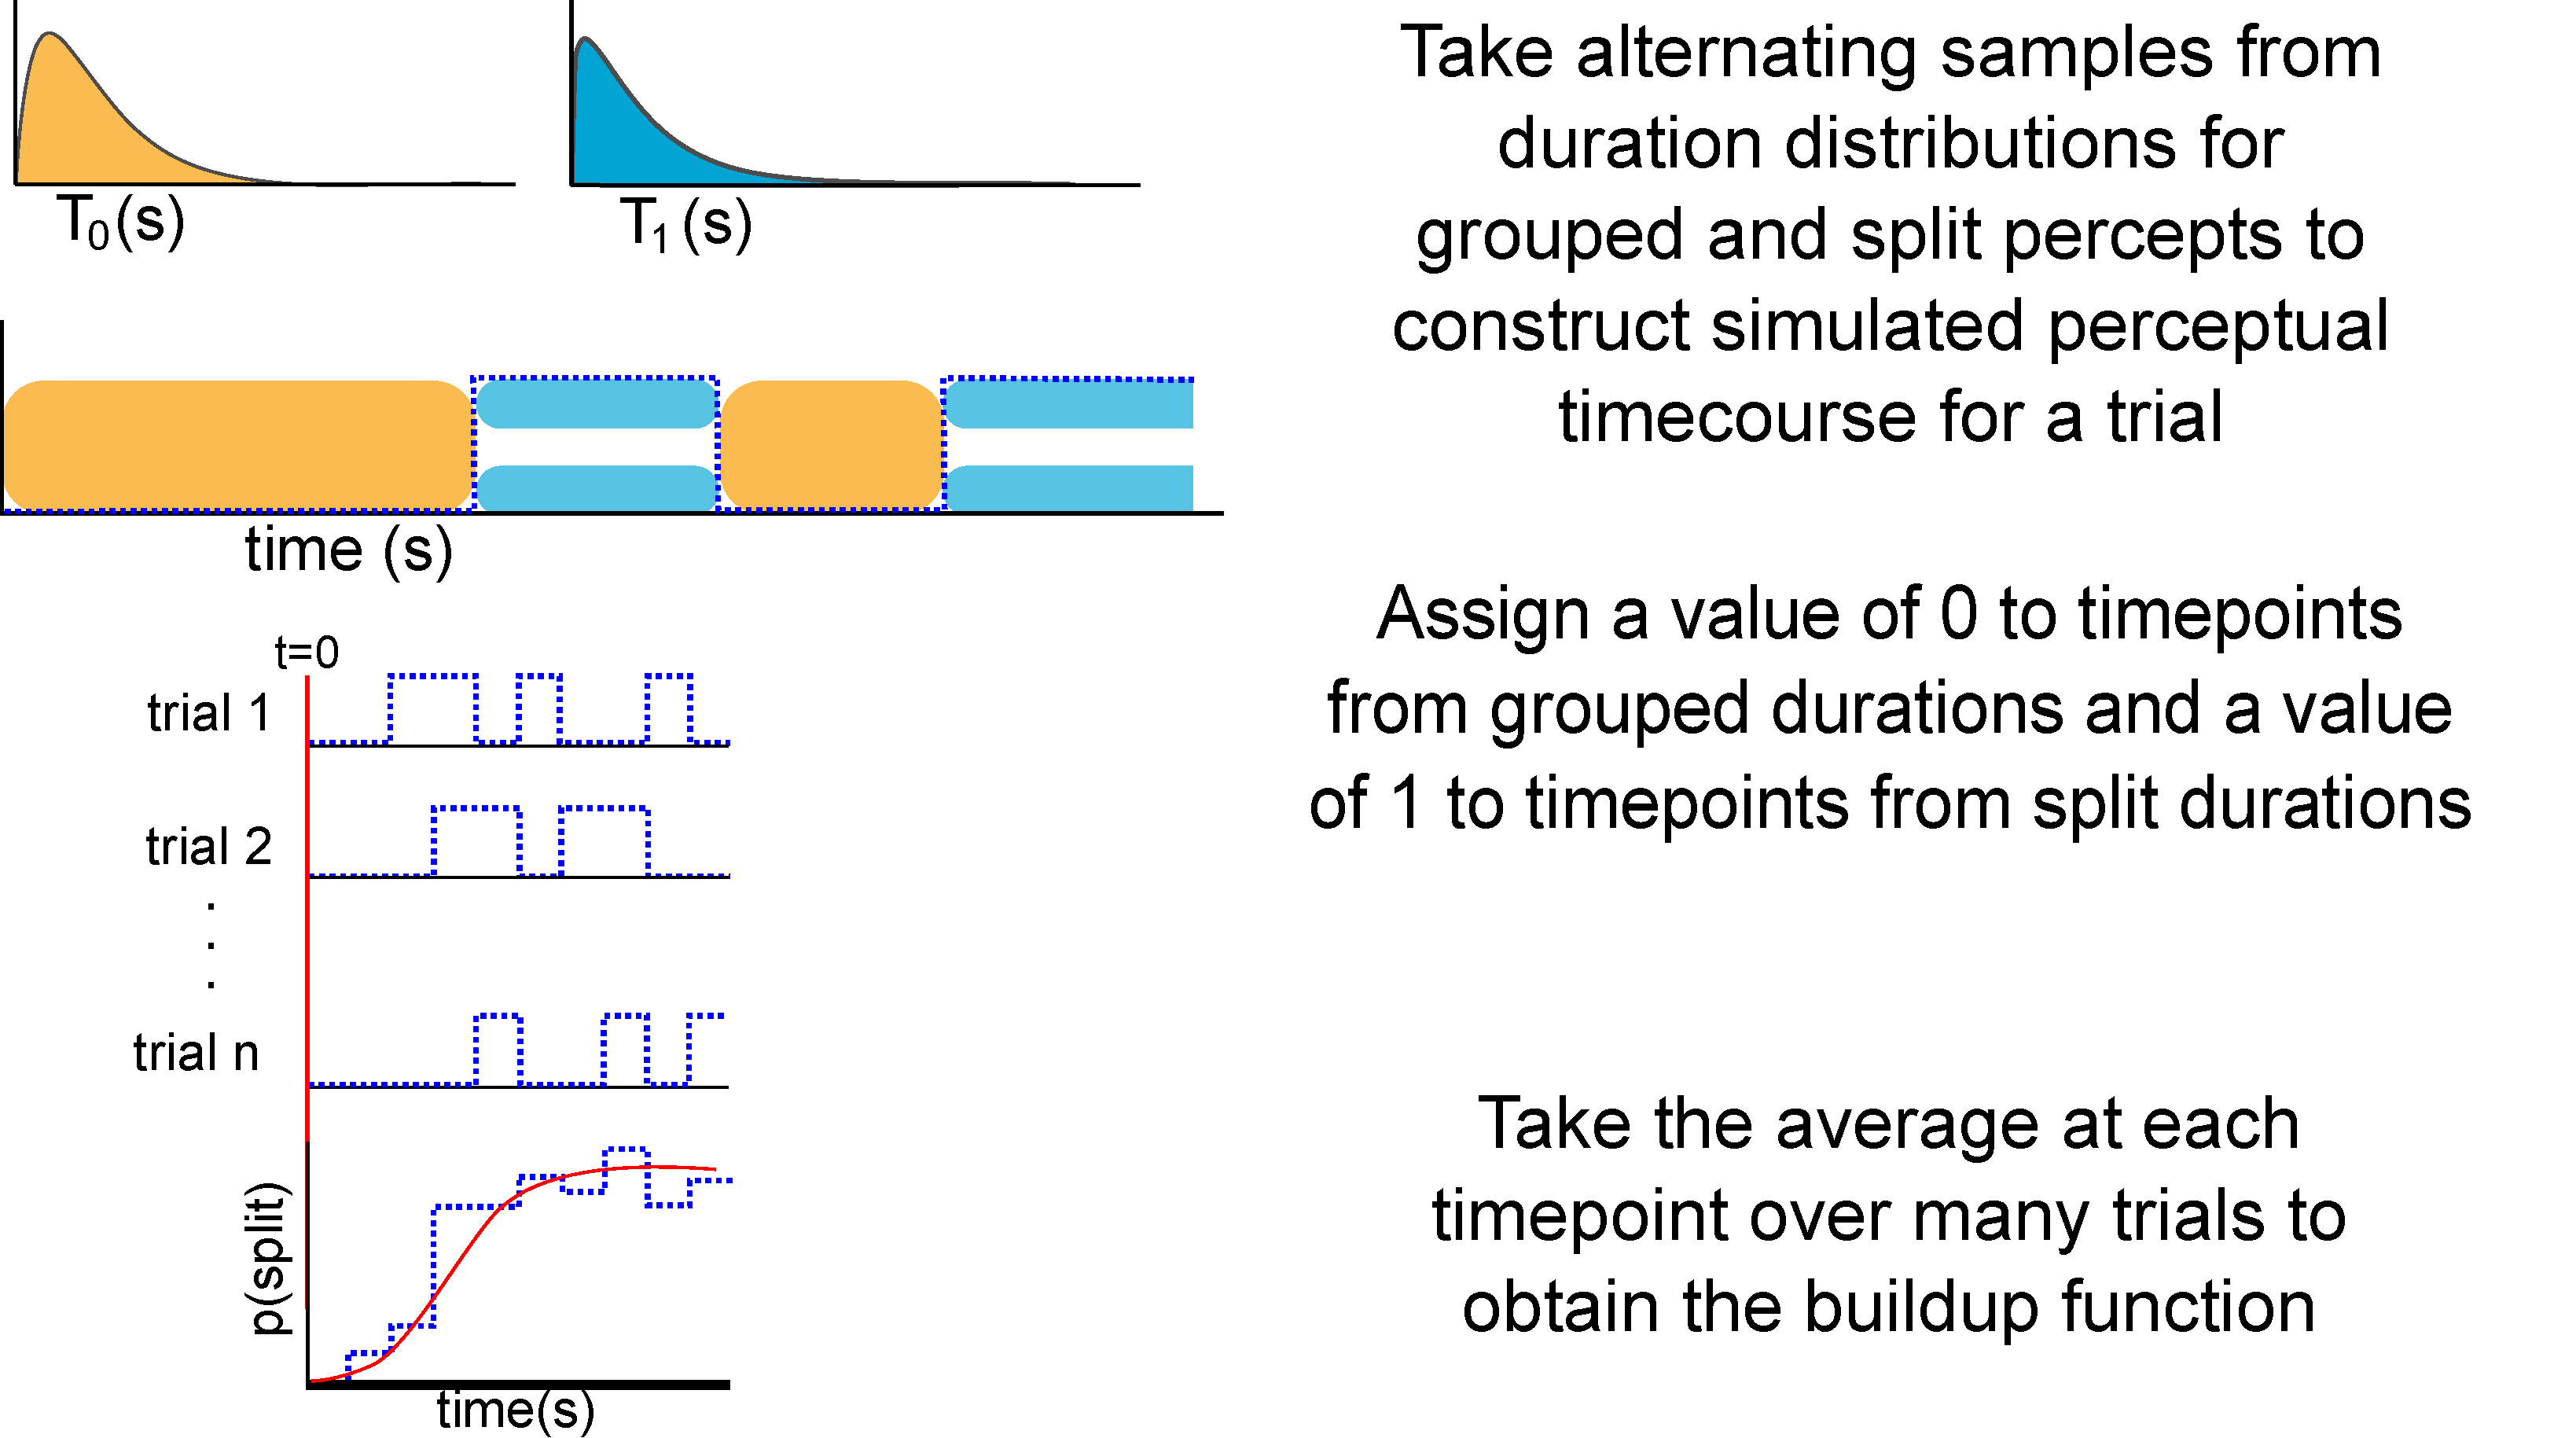
\includegraphics[width=0.75\textwidth]{../percepts&distributions&BUF}} \\
	  \vspace{20 pt}
      \sidesubfloat[]{\label{fig:b}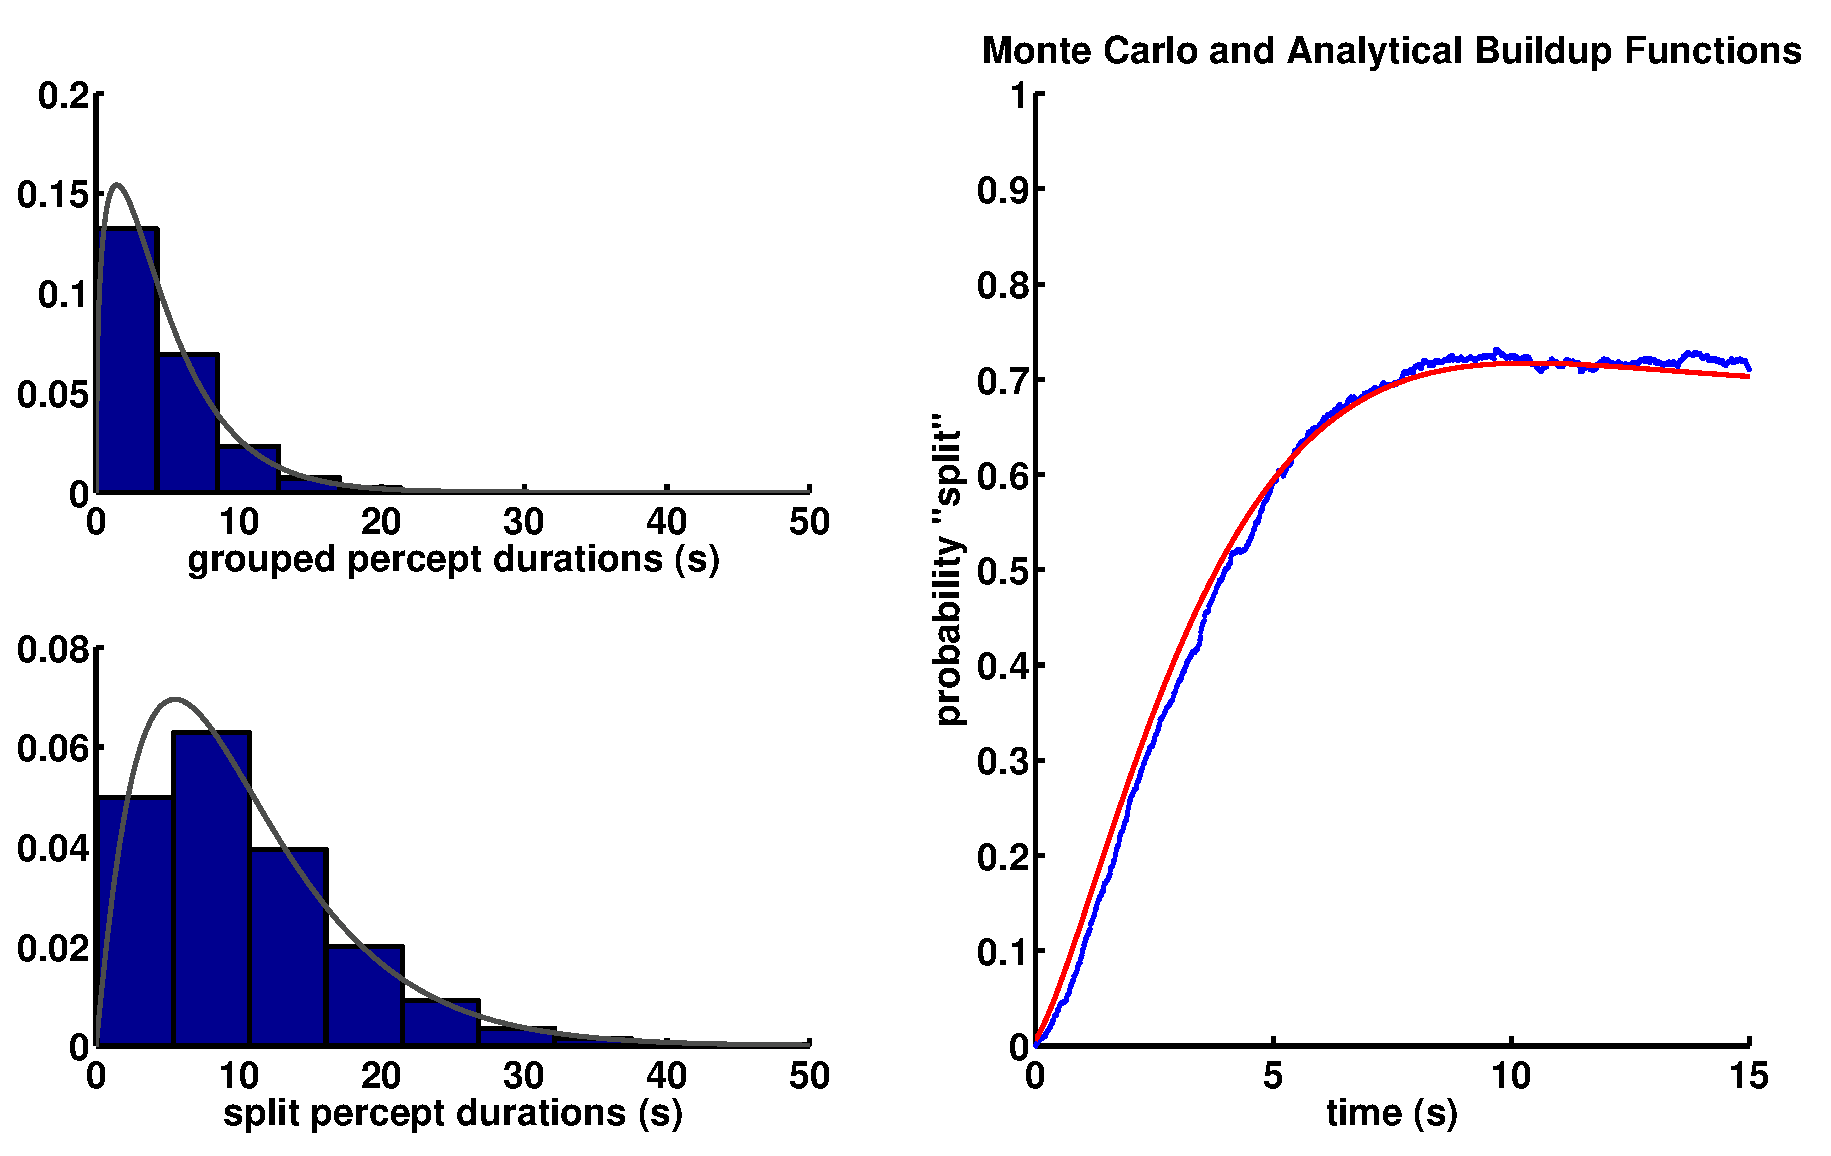
\includegraphics[width=.9\textwidth]{../monte_carlo_convergence}}
   
	\caption{\textbf{(a)} Visualization of the alternating renewal process producing a buildup function. We used gamma probability density functions approximating duration distributions to construct Monte Carlo simulations. The analytical solution to the alternating renewal process model, shown as a red solid curve (bottom), allows us to predict buildup as a function of the distributions of dominance durations of each of the perceptual states. \textbf{(b)} Monte Carlo simulation computed buildup function of 1000 trials (blue) approaches the theoretical solution (red). Gamma distribution parameters chosen from fits to a preliminary psychophysical dataset (not shown).}
	\label{fig:makingBUFs}
%\end{wrapfigure}
\end{figure}

We initially tested this theory in Monte Carlo simulations by simply constructing in silico perceptual timecourses according to the above assumptions (see Figure \ref{fig:makingBUFs}, (a)). For a given simulated trial timecourse, we draw alternating random samples from each of two distributions-- one corresponding to the grouped state durations, and the other to the split state durations. We draw the first sample from the distribution corresponding to the grouped state, the second from that corresponding to the split state, and continue drawing samples from each distribution in alternation until the sum of all the durations exceeds the length of a trial. These trial durations are converted into discretized timecourses by assigning a value of 0 to time intervals during which the state corresponds to a grouped percept, and assigning a value of 1 to the time intervals for which the percept state was split. In Monte Carlo simulations, we produce an arbitrarily large number of such trial timecourses, then take the average at each time point. This simple process, with no history dependence between successive samples, produces buildup-like curves.

We have also derived an analytical solution to this process using a population density approach similar to that used in \cite{Stinchcombe2012} to model stochastic gene expression. There are a number of advantages to characterizing the buildup function in this way. First, with an analytical solution relating the distributions of durations for grouped and split percepts to the buildup function, it is theoretically possible to interconvert between buildup functions and the statistics of the dominance durations for each percept. We have developed this solution into a statistical switching model to reconstruct the buildup function from four parameters- the parameters for the gamma densities for grouped and split percept durations. This theoretical solution coincides with the Monte Carlo simulation results  (see Figure \ref{fig:makingBUFs}b). This is convenient, as the analytical solution is computationally less expensive than iterative Monte Carlo simulations, and the solution is exact. Furthermore, in the alternating renewal process framework, there is no explicit mechanism of accumulation. Therefore, this formulation challenges the conventional understanding by which computing the buildup function of sound source segregation as requiring a gradual accumulative process.

\subsection{Competition model simulations produce buildup as a consequence of alternations} 

There has been a great deal of work done to understand the neural computations that could underlie perceptual alternations with ambiguous stimuli. Previous investigations (\cite{Wilson1972, Wilson2003, Laing2002, Shpiro2009, Pastukhov2013}) have used population firing rate models with competition architecture to model perceptual bistability. In these pseudoneuronal mutual inhibition models, there are separate populations whose firing rates represent the perceptual strength of each interpretation of the stimulus. They make inhibitory connections onto one another, so the population with the highest firing rate typically dominates the other. These models were originally developed to describe binocular rivalry, but have also been used to account for the psychophysical results of experiments with ambiguous grouping-- namely, moving plaids with coherent/transparent motion (\cite{Shpiro2009, Laing2002, Pastukhov2013}) and triplets with streaming integration/segregation (\cite{Mill2013}).

In competition models, the relative firing rates of the two populations are taken to produce the simulated observer's perceptual reports. The population with the higher firing rate corresponds to the dominant percept. Because the two populations mutually inhibit each other, in most cases only one population is active at any given time. In addition, each population undergoes adaptation in response to its own firing rate. The alternation of dominance epochs between the two populations can be driven by two mechanisms. If adaptation is strong enough, then the activity of the dominant population will decay over time, while the suppressed population recovers from any prior adaptation. This leads to periodic alternations between dominance states with oscillation dynamics. However, if adaptation is weak, the system will display attractor dynamics, in which alternations are driven by noise in the externally applied inputs. The brain appears to be a very noisy system, with random fluctuations occurring at multiple scales such as vesicular release and spiking variability.

The difference between oscillator and attractor dynamics in these competition models is most simply understood by observing how the system would behave without noise (\cite{Shpiro2009, Moreno-Bote2007}). For oscillation dynamics, adaptation would cause the dominant population to reduce its activity over time, reducing the inhibition on the suppressed population, allowing it to become active. In a noiseless system, stable fixed points in the system appear and disappear over time, and alternations will occur deterministically with a constant period. Noise in such a system will affect the distribution of dominance durations for each state, but is not required for switching. Conversely, attractor dynamics occurs when a system has multiple stable states at the same time. In the absence of noise, the initial conditions determine which state becomes active, and the system behaves in a winner-take-all fashion. That is, the population that becomes dominant first is permanently active, and the other population is permanently suppressed. However, injecting noise into such a system can cause switches from one stable state into another. In this case, the switching between perceptual dominance states would be caused by the noise itself. 

\floatsetup[figure]{style=plain,subcapbesideposition=top}
\begin{wrapfigure}{L}{.6\textwidth}
	\centering
	\sidesubfloat[]{\label{fig:a}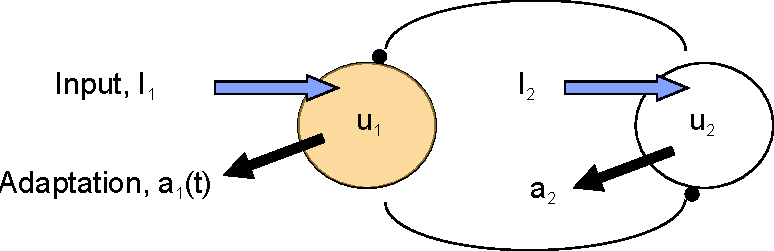
\includegraphics[width=0.5\textwidth]{../comp_model}} \\
	\vspace{20 pt}
	\sidesubfloat[]{\label{fig:b}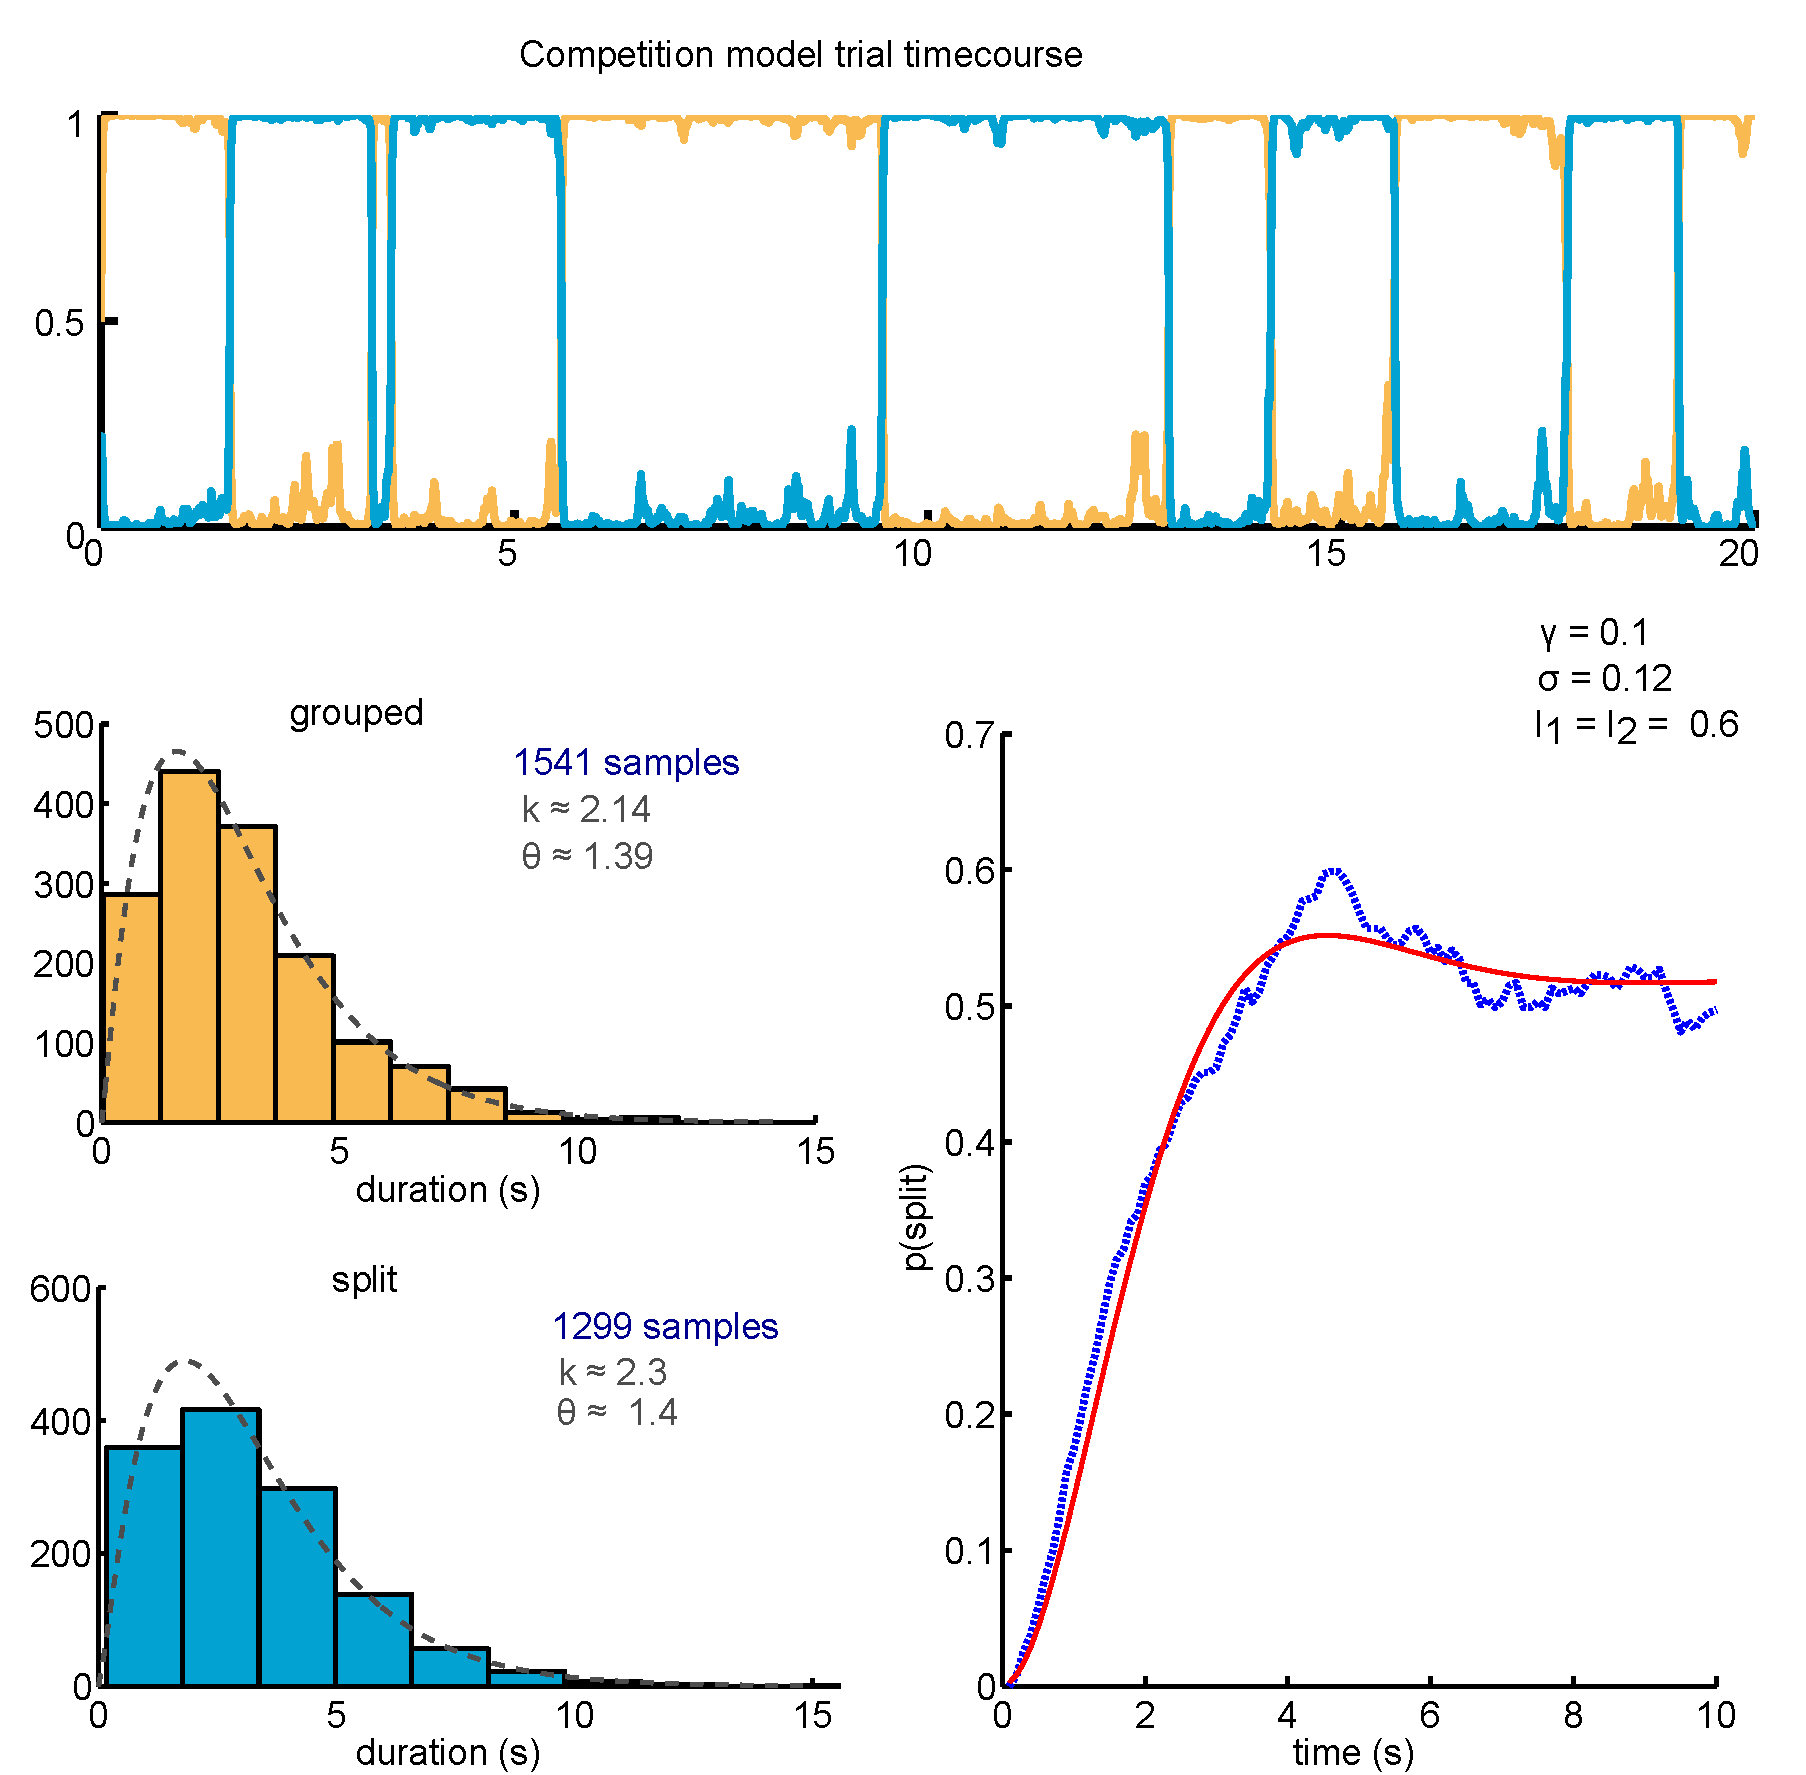
\includegraphics[width=.9\textwidth]{BUFs_hists_lowadapt}} 
	
	\caption{\textbf{(a)} Mutual inhibition population firing rate model producing buildup. We choose initial conditions to ensure that the population representing the grouped percept, $u_1$, is always dominant at the beginning of a given trial timecourse. \textbf{(b)} Competition model simulation results for parameters that produce attractor dynamics with noise-driven switching. Top, population activity timecourse for one 20-second trial. We simulated 500 trials to produce the buildup function, lower right (blue). Histograms of the dominance durations, with maximum likelihood estimated gamma density parameters and the associated density functions (gray), are shown in the lower left. These parameters allow us to compute analytically the resulting buildup function for an alternating renewal process (red).  The buildup function looks similar to those reported in the psychophysical literature, and the statistical model's prediction is good (R-Squared = 98\%).}
	\label{fig:making_comp_BUFs}
	%\vspace{-20 pt}
\end{wrapfigure}

We wanted to use the competition model as a test-bed for the theory of the alternating renewal process. We chose initial conditions that ensured that the grouped percept was always dominant at the beginning of the trial, as our hypothesis that alternations could produce buildup relies on this assumption. We did this in a very simple manner (see Figure \ref{fig:making_comp_BUFs}), by setting the initial condition on the population representing the grouped percept to half its maximum value. All other initial conditions were set to 0. From the population firing rates we computed dominance durations, which were converted to binary timecourses and averaged over trials to produce competition model buildup functions. Using this method, we produced buildup functions for both oscillator and attractor competition models.

To test the application of the alternating renewal process model, we viewed dominance durations of each state from the short simulated trials as samples from underlying gamma distributions. Because our competition model simulations generated trials that were only 20 seconds long, a large proportion of these durations were truncated by the end of the trial. We estimated gamma parameters $k$ and $\theta$ that maximized the likelihood of the complete as well as the right-censored dominance durations for each model perceptual state. Using only the four parameters so obtained, we were able to get very strong fits to the buildup function (R-squared $>$ 90\%).

\subsubsection{Psychophysically observed buildup is inconsistent with oscillator-driven alternations}

\begin{wrapfigure}{L}{0.5\textwidth}
		\centering
		
		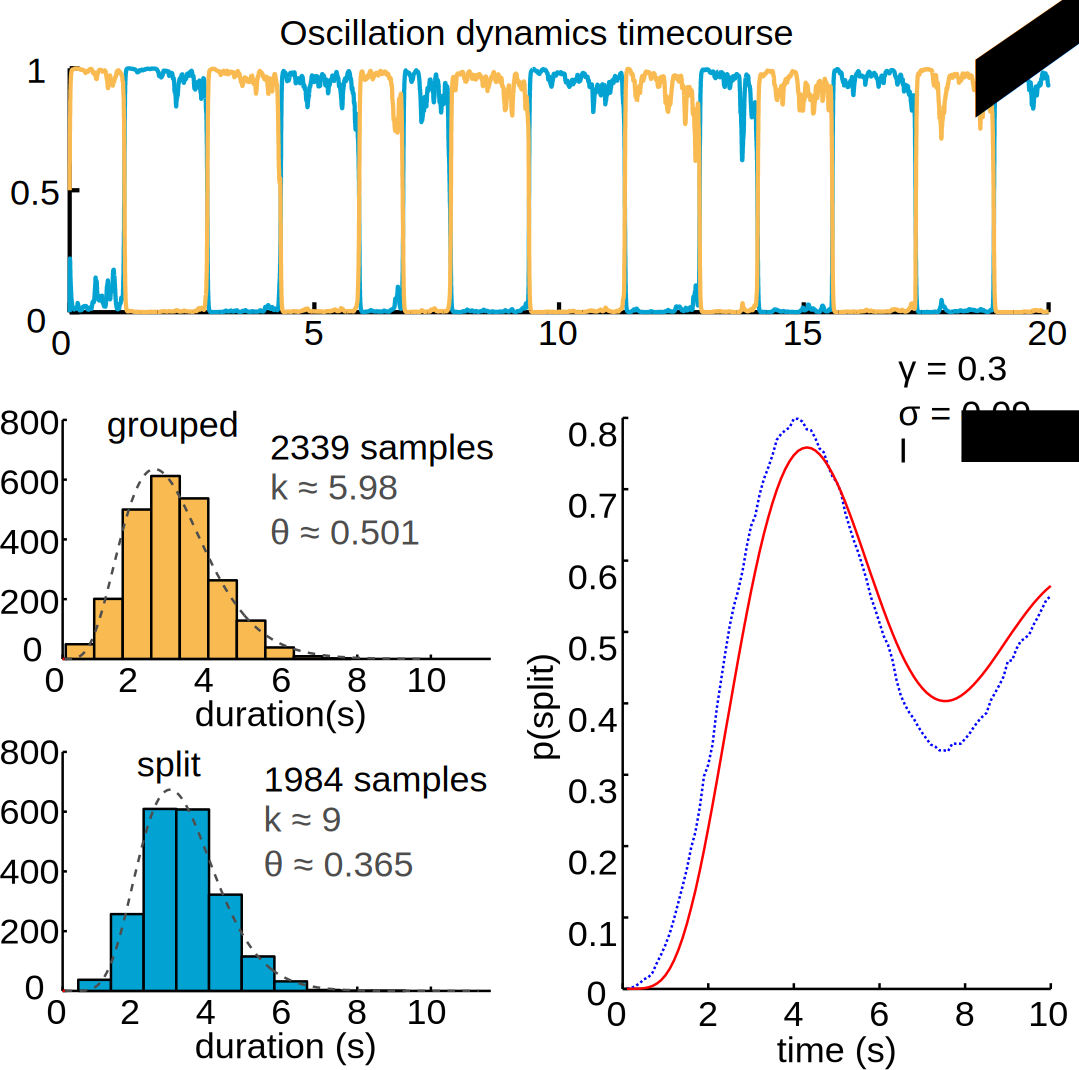
\includegraphics[scale=.24]{hi_adapt_low_noise_equal_inputBUFsHists}
				
		\caption{Competition model simulation results for parameters that produce oscillation dynamics with adaptation-driven switching. Top, population activity timecourse for one 20-second trial. The dominance durations are much more regularly timed than those produced under attractor dynamics, reflecting the clock-like periodicity of the underlying oscillator. These oscillations are dramatically present in the average over 500 simulated trials, lower right (blue). To our knowledge, no such buildup functions have been observed psychophysically. The maximum likelihood estimated gamma density parameters are shown in the lower left (gray), and the analytically computed buildup function for an alternating renewal process with those parameters is shown in the lower right (red). The fit between the analytical solution and the trial average is still quite good (R-squared = 93\%).}
		\label{oscillation_dynamic_buildup}
\end{wrapfigure}


Previous work from our lab has shown that oscillation dynamics are inconsistent with a number of statistical features of the dominance durations reported in psychophysical experiments (\cite{Shpiro2009}). The mean and circular variance of dominance durations under these dynamics do not fall within the range of those observed for perceptual reports of ambiguous visual displays. Furthermore, when adaptation drives alternations in the dominance of population activity, we observe moderate and significant correlations between successive percepts. Data from the psychophysical literature suggests that the durations of subsequent percepts are only weakly correlated, if at all (\cite{Pressnitzer2006}).

We wanted to examine buildup under each of these dynamical regimes in order to determine whether we could find correspondence between the buildup functions produced by competition models and those reported in the psychophysical literature. Previously reported psychophysical data indicate that the buildup function is monotonic. To our knowledge, no psychophysical experiments have shown a buildup function timecourse with a damped oscillatory approach to steady state. Buildup functions produced under oscillation dynamics in our competition model (Figure \ref{oscillation_dynamic_buildup}), however, display damped oscillations reflecting the underlying periodicity of the mechanism of alternation from the oscillator regime. As previously reported \cite{Shpiro2009}, these buildup functions are derived from perceptual timecourses for which there are significant correlations between successive percept durations, such that the present perceptual state depends on the cumulative history of previous percepts. Although the correlation coefficient between durations of subsequent percepts was significant (r = 0.23), the fit to the buildup function by finding the parameters of density functions for long term percept durations was strong ($R^2 = 93\%$). Despite ignoring history dependence, the theory linking buildup to long-term dynamics gives accurate predictions. 

\floatsetup[figure]{style=plain,subcapbesideposition=top}
\begin{figure}
	\centering
	\sidesubfloat[]{\label{fig:a}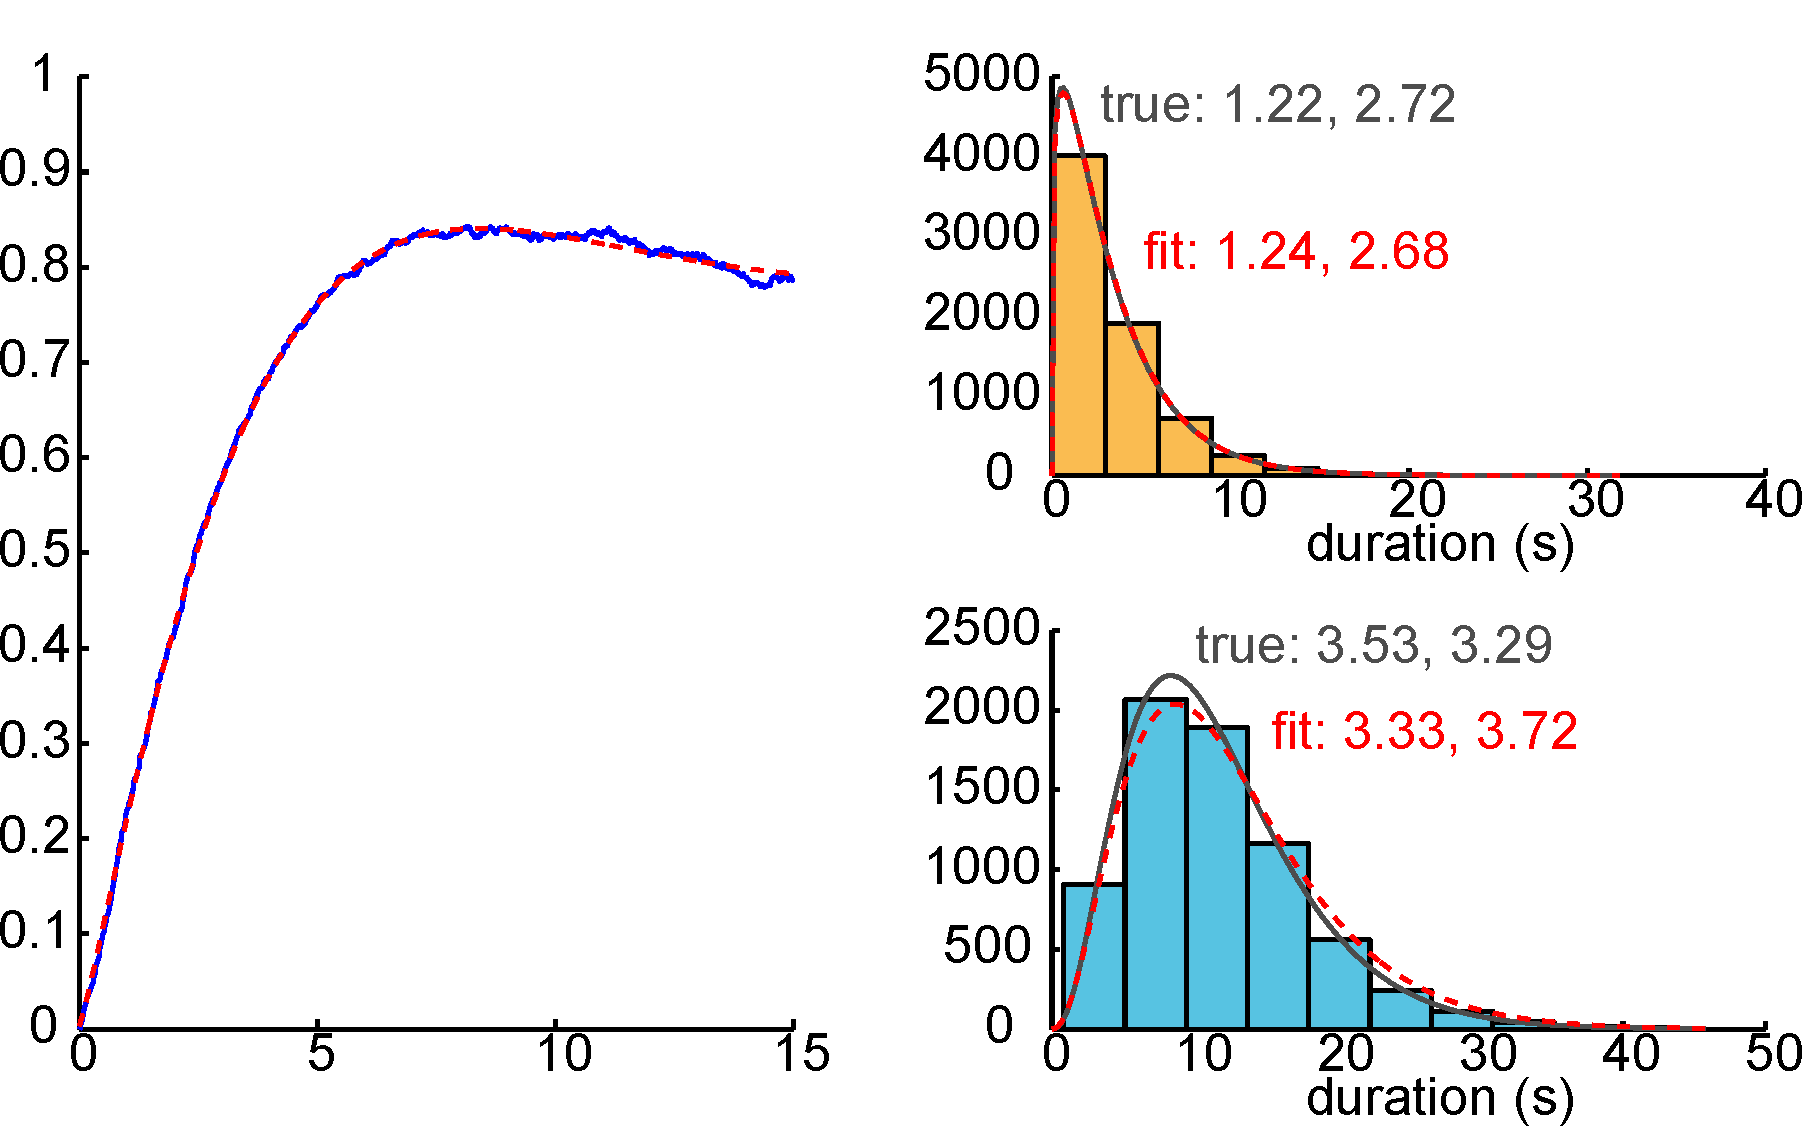
\includegraphics[scale=.35]{../4par_reverseGood}} \\
	\vspace{20pt}
	\sidesubfloat[]{\label{fig:b}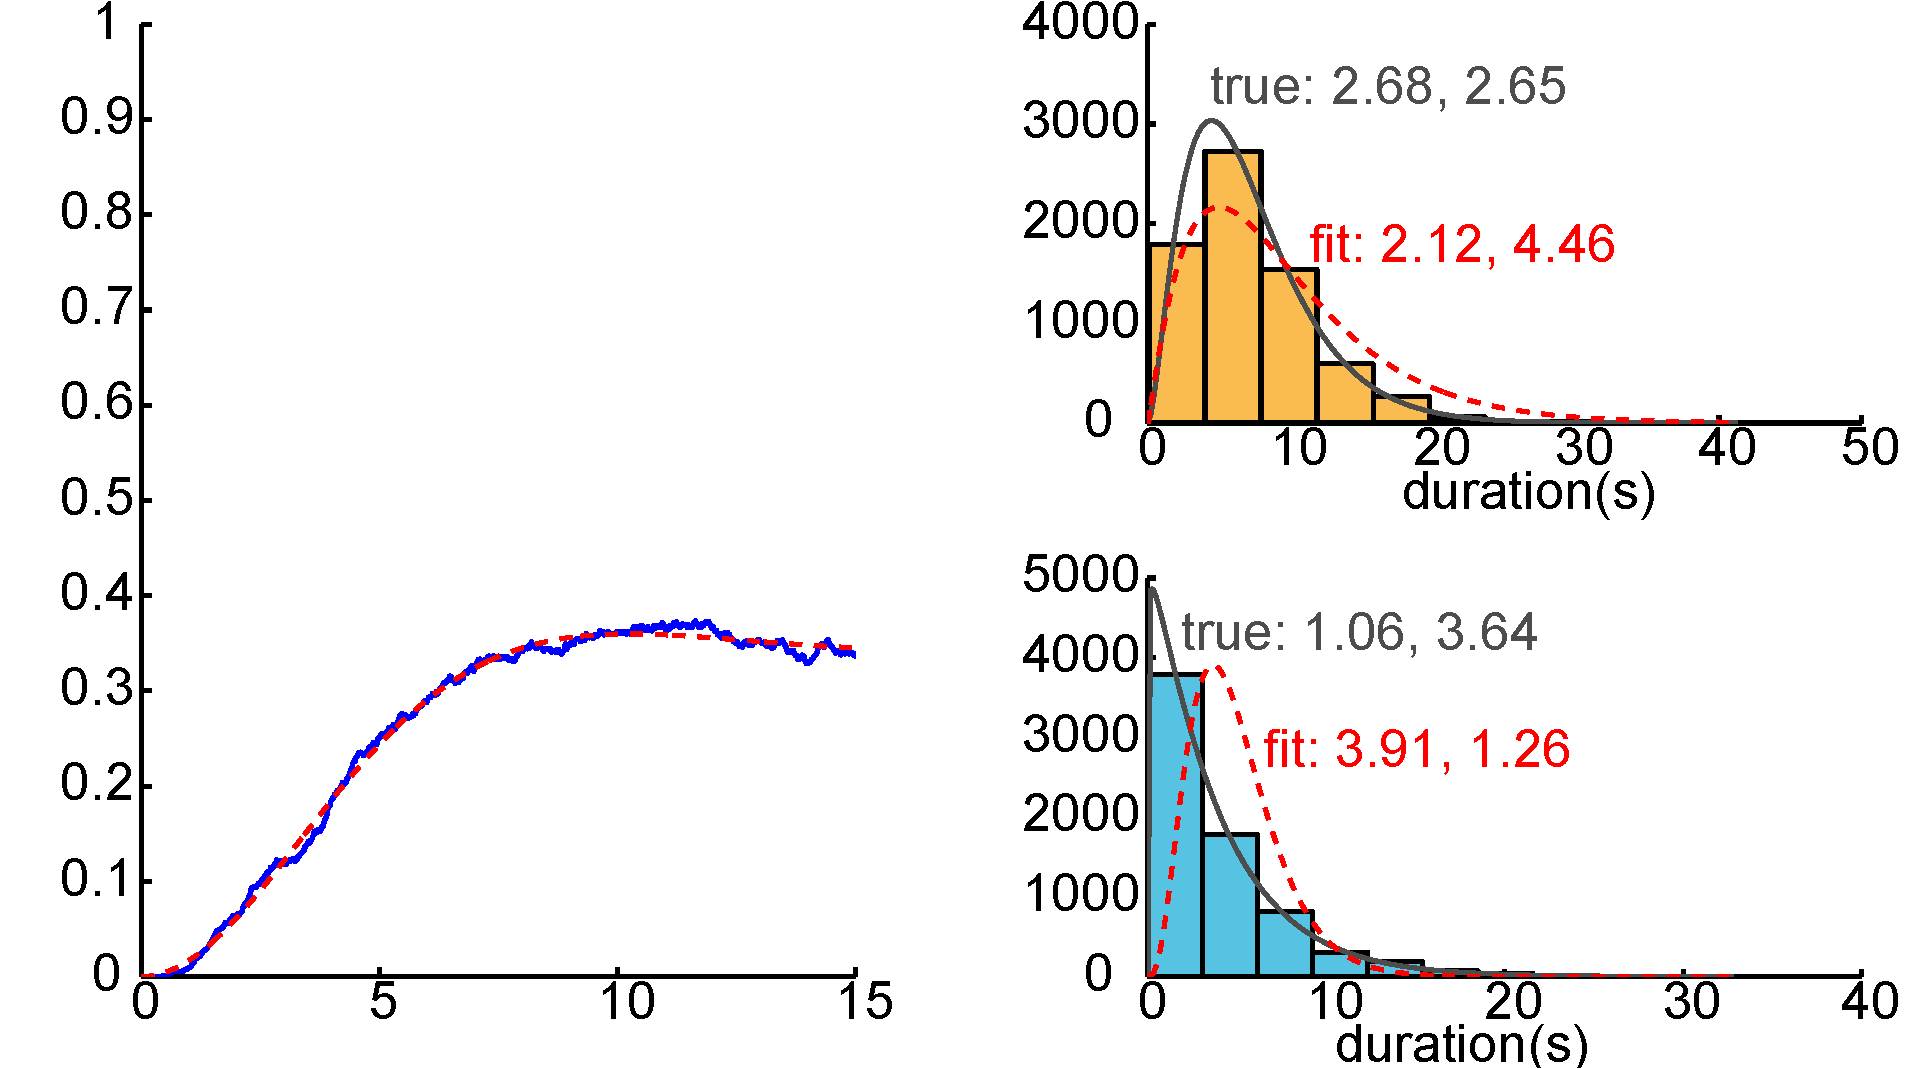
\includegraphics[scale=.35]{../4par_reverseBad}}
	
	\caption{We generated buildup functions, shown in blue, with Monte Carlo simulations from known gamma densities (shown in gray on the histograms). We then obtained estimates for those parameters by finding the least squares fit to the Monte Carlo simulated buildup functions from our four parameter analytical expression. The fitted buildup function and the gamma densities so recovered are shown in dashed red lines. \textbf{(a)} A successful recovery of the gamma density parameters from the buildup function. \textbf{(b)} One case in which the parameters that minimize squared error between the analytical and the Monte Carlo simulated buildup function do not match the underlying gamma densities used to produce it.}
	\label{fig:reverse_fit_4par}
\end{figure}

\subsection{Duration distributions are not well constrained by the trial average}

The resilience of the alternating renewal process to capture the dynamics of buildup in a variety of circumstances, including those with duration-to-duration correlations, likely carries the burden of overflexibility-- for any given buildup function, a wide range of pairs of distribution functions may provide a good fit. We generated buildup functions using Monte Carlo simulations as in Figure \ref{fig:makingBUFs} and used our analytical solution to find the gamma density parameters that minimized the squared error between the Monte Carlo simulated and analytical buildup functions using an alternating renewal process with those underlying gamma density parameters. In general, the parameters so found did not strongly fit the histograms of the duration samples used (see Figure \ref{fig:reverse_fit_4par}).
Specifically, we used one-sample Kolmogorov-Smirnov tests to determine whether the duration samples came from the gamma distribution obtained from the least squares fit to the buildup function. Only 24.5\% of simulations produced good fits, and the average KS distance between sample and the fitted distribution was .09.

However, for the special case when the both perceptual states have identical duration distributions, the parameter estimation for the gamma density functions from the buildup function is much better. This circumstance occurs in competition model simulations when the inputs to the populations representing each percept are matched, e.g., when the stimulus is perfectly ambiguous. We generated buildup functions using Monte Carlo simulations from two identical gamma densities, and found the single pair of gamma parameters that minimized squared error between this and theoretical buildup function (Figure \ref{fig:2par_reverse_fit}). For 1000 such simulations, 63\% of the recovered parameters were indistinguishable from the sample empirical distribution by Kolmogorov-Smirnov tests, and in general the fits were much closer, with a mean KS distance of .04. This method of estimation may prove useful for providing at least a rough estimate of the duration distributions underlying steady state switching dynamics.

\section{Discussion}
\subsection{What if the first percept is longer?}

One issue we have not addressed so far in our presentation of the alternating renewal process model is inertia (\cite{Hupe2012}). For ambiguous displays, the time until the first perceptual switch is typically much longer than subsequent durations of the same percept. For stimuli with ambiguous grouping, the distribution of initial grouped percept durations is different from other grouped percepts. In some experimental data collected with short trials, this might not be especially concerning-- most trials contain one or fewer switches, i. e., from the integrated to the segregated percept. With these data, the distribution of initial switch times would be sufficient to describe a renewal process accounting for buildup. For data collected from longer trials with many alternations, however, it might be desirable to distinguish between initial and subsequent grouped percept durations. Our theoretical model is capable of computing the buildup function from both steady state and initial percept distributions; however, this would introduce a third duration distribution, and increase the number of parameters to 6. For simplicity's sake, we have only shown the 4 parameter model, which assumes that the initial percept duration is drawn from the same distribution as other grouped percept durations.

To adequately explain these perceptual dynamics with a physiological model, there should be some description of the sensory coding mechanisms that underlie the formation of perceptual organization. The specific mechanisms for switching in human stream segregation may be complex; (\cite{Kondo2009}) find that feedforward and feedback processes in a thalamocortical loop might be differentially engaged for switches into and out of the perceptual organization that is strongest. The renewal process model is agnostic to the specific mechanism by which states are found and alternations occur; we have used existing competition models for the sake of illustration and as a computational test-bed. Similar competition-like processes have been used to explain the alternations observed in ambiguous motion \cite{Pastukhov2013} and stream segregation (\cite{Mill2013} experiments). A better understanding of the characteristics of the neural populations on the encoding side of perceptual organization could enable us to more accurately model the psychophysical data.
 .
%Our competition model, as it stands, produces a different distribution for initial and subsequent grouped percepts. However, the initial percepts are shorter in mean duration. This can probably be fixed by using a different set of initial conditions to achieve the correct initial dominance state-- for instance, by setting the initial conditions so that the other population, that which represents the split percept, is highly adapted at the beginning of the trial. However, such an approach would be arbitrary, and leaves something to be desired in terms of explanatory value. What would be better is a more detailed model that captures elements of the sensory coding and neural dynamics that produce the perceptual states in the first place. For instance, percept formation might be subserved by neural populations that respond only to particular spectrotemporal input patterns. These encoding neural populations would be subject to adaptation, etc, and could allow us to make predictions about the perception of novel stimuli.


\begin{wrapfigure}{L}{0.6\textwidth}
	\centering
	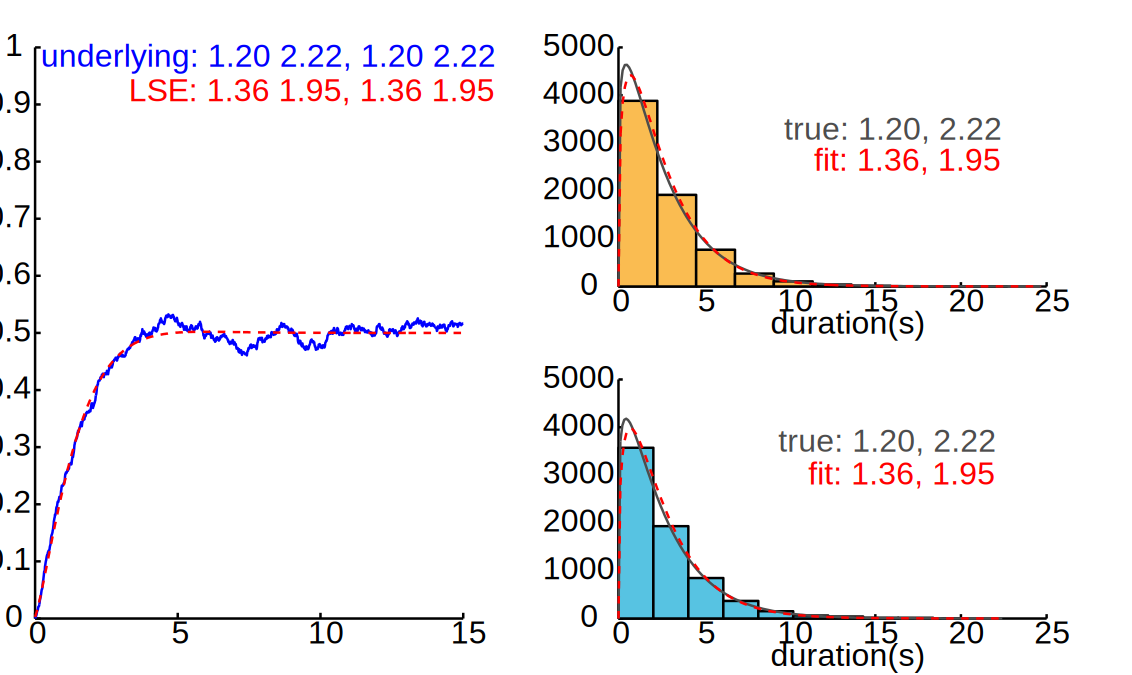
\includegraphics[scale=.35]{../2par_reverse}
	\caption{The same as Figure \ref{fig:reverse_fit_4par}, except that the Monte Carlo simulations have been constrained so that the gamma densities for each of the two states are matched. In addition, the least squares fit is constrained to find only two parameters. The recovered parameters for the duration distributions usually match those used to generate the Monte Carlo simulated buildup function.}
	\label{fig:2par_reverse_fit}
\end{wrapfigure}



Our theoretical solution can be modified to account for experimental data in which the initial percept duration distribution is different from the steady state. However, there are circumstances in which inertia is fairly trivial, such as when buildup resets after a switch in attention (\cite{Denham2010}). Stationary distributions might be appropriate for such circumstances. We can take a more abstract view and consider a steady-state buildup function constructed from averaging over timepoints aligned by switches into the grouped percept.

To address the issue of inertia and the longer mean duration of the initial percept than subsequent grouped percepts on a trial, we considered a new method for constructing the buildup function: switch-triggered averaging. This method allows us to produce a buildup function from a single long trial. Discarding the first and second percept duration, we can construct buildup functions by estimating the probability over time for the split percept based on an event-triggered average aligned to each switch into the grouped percept. This method produces a buildup function at steady state, the probability of perceiving the split organization not just from the beginning of the trial but rather from the beginning of any switch into the grouped perceptual organization over the course of a long presentation. 

\subsection{Do percept-to-percept correlations matter for describing buildup?}

The previous competition model simulations provide a test-bed for our novel statistical model. When dominance durations are not statistically independent, and there is history dependence between successive perceptual epochs, will modeling the buildup function as an alternating renewal process with state durations from underlying independent gamma densities still provide a good description? We measured the correlations in the data produced for both a noise-driven and adaptation-driven alternation dynamics. As previously described, the adaptation-driven perceptual timecourses showed moderate correlations between the durations of successive percepts. Our statistical model, however, ignores this history dependence entirely, treating percept durations as independent random variables described by their probability density functions. The buildup functions so computed matched the buildup function computed from the output of the neuronal competition models. Correlations between subsequent perceptual epochs do not need to be taken into consideration to predict the buildup function; rather, these perceptual dynamics are described sufficiently well by the underlying distributions of dominance durations.
%While we do not explicity invoke an accumulative process to describe this switch, the use of a gamma density to describe the distribution of dominance durations for the grouped percept implies history dependence. This is because the hazard function for a gamma density, in contrast to an exponential distribution, is dependent on time elapsed, evolving from 0 at time zero to a steady state value. The time dependence of the probability of switching out of the grouped percept may therefore be complementary with previous descriptions. 

Previous computational approaches to describing the buildup function (\cite{Micheyl2005, Pressnitzer2008}) have pointed to the accumulation of adaptation as a critical feature for the increase over time in the probability of a split percept. Multi-second habituation in the auditory periphery (\cite{Pressnitzer2008}) can predict the buildup function obtained through psychophysics. It may therefore be surprising that the alternating renewal process neglects to account for adaptation. We believe that previous approaches and our own can be reconciled, and may even be complementary. The choice of gamma densities to generate dominance durations implicitly invokes adaptation (\cite{Wilbur1982}). This is because the hazard function for a gamma density, in contrast to an exponential distribution, is dependent on the time elapsed, evolving from 0 at time zero to a steady state value. The time dependence of the probability of switches from the grouped to the split perceptual organization may therefore be seen as complementary with the habituation-based explanation for the buildup function. 

What is still missing from these theories, however, is the mechanism by which the perceptual state switches back and undergoes alternations; how do we account for switches out of the split percept? Our statistical model is agnostic to the mechanism of switching, but it does use information about alternations to predict perceptual dynamics. This is a novel insight linking transient dynamics to any underlying steady state process generating alternations, and produces surprisingly good predictions with minimal assumptions.



%single switch case is just a distribution of integrated percept/first switch times and a distribution of split percept durations that is centered at a mean far exceeding the time course of data collection.\\
%sequence detector\\
%our statistical model is good

\subsection{Summary}
We have presented a statistical model that explains how the distribution of state durations for an alternating renewal process at steady state describes the system's behavior before reaching steady state. 

\subsection{Data Sharing}

Frontiers supports the policy of data sharing, and authors are advised to make freely available any materials and information described in their article, and any data relevant to the article (while not compromising confidentiality in the context of human-subject research) that may be reasonably requested by others for the purpose of academic and non-commercial research. In regards to deposition of data and data sharing through databases, Frontiers urges authors to comply with the current best practices within their discipline.

\section{Material \& Methods}

\subsection{Derivation for alternating renewal process}
In the alternating renewal process there are 2 random variables, S(t) and Z(t). S(t) is the random elapsed time since last switching into the current state, evaluated at time t. Z(t) is a dichotomous random variable, where Z(t) in ${0,1}$ codes for the percept, grouped or split. For sake of convenience, we introduce 2 probability density -mass functions: $f_0(s,t) ds = Pr \lbrace S(t) \rbrace$ in $(s,s+dt)$ and $Z(t)=0$, and $f_1(s,t) ds= Pr(S(t)$ in $(s,s+ds)$ and $Z(t)=1$. The coupled pair of partial differential equations describing the evolution over time of these 2 probability density-mass functions is as follows:
%The solution to the alternating renewal process was implemented by solving a set of probabilistic differential equations describing the rate of change in probability per unit time for each of the two states of a dichotomous random variable $Z(t) = {0 , 1} $, as follows:

\begin{equation}
\frac{\partial f_0}{\partial t} \big(s,t\big) = -\frac{\partial}{\partial s}\big(1 * f_0(s,t)\big) - h_{T_0}(s) f_0(s,t)
\end{equation}

\begin{equation}
\frac{\partial f_1}{\partial t} \big(s,t\big) = -\frac{\partial}{\partial s} \big(1 * f_1(s,t)\big) - h_{T_1}(s) f_1(s,t)
\end{equation}

where $s$ is the elapsed time since entering state $i$ and $h_{T_i}(s)$ is the hazard function, the probability per unit time of exiting the current state at time $t$. $h_{T_i}(s) = \dfrac{f_{T_i}}{\hat{F}_{T_i}}$, the ratio of the density function of durations $T_i$ for state i and its complementary cumulative distribution function.

The value of $S(t)$ is reset to 0 whenever an alternation between states occurs. The initial flux of probability (a source) at s = 0 is determined by the probability of switches out of the previous state, leading to the following boundary conditions:

\begin{equation}
f_0(0,t) = \int_0^\infty h_{T_1}(s) f_1(s,t) ds
\end{equation}

\begin{equation}
f_1(0,t) = \int_0^\infty h_{T_0}(s) f_0(s,t) ds
\end{equation}

The probability that $Z(t)=1, p_1(t)$, is the marginal probability mass function evaluated at $z=1$. It is obtained by integrating $f_1(s,t)$ over all s; and similarly for $Z(t)=0$.
We used the following initial conditions, corresponding to $Pr \lbrace Z(t=0)=1 \rbrace=1$, and $Pr \lbrace Z(t=0)=0 \rbrace = 0$. In order to allow for a different distribution for the initial percept, we first solve for the case of beginning in state 1:

\begin{equation}
f_1(s,t=0) = \delta(s); f_0(s,t=0) = 0
\end{equation} 

For sake of simplifying notation, we define $p_{1|1}(t)=Pr \lbrace Z(t)=1|Z(t=0)=1 \rbrace$. Using these conditions yields the following solution:

\begin{equation}
p_{1|1}(t) = \tilde{F}_{T_1}(t) + \frac{1}{2\pi} \int_{-\infty}^\infty dw \frac{1}{i\omega} \left[ \hat{\tilde{F}}_{T_1}(\omega) \hat{f}_{T_0}(\omega)\hat{f}_{T_1}(\omega) \frac{i\omega}{1 - \hat{f}_{T_0}(\omega)\hat{f}_{T_1}(\omega)} \right] e^{i \omega t}
\end{equation}
where $\hat{f}(x)$ is the Fourier transform of $f(x)$

To find the probability that $Z(t)=1$, given $Z(t=0)=0, p_{1|0}$, we time shift the above expression by the durations of the initial state, $T_0^0$, whose density function is $p_{T_0^0}(t)$ [changed f to p]. This amounts to a convolution of the density for initial durations (and first switch times) with the previous solution:

[again changed f to p]
\begin{equation}
p_{1|0}(t) = \int_0^t f_{T_0^0}(s) f_{1}([t-s]|z(0)=1) ds
\end{equation}

Thus the solution can be given in the Fourier domain as:
\begin{equation}
\hat{p}_{1|0}(\omega) = \hat{f}_{T_0^0}(\omega) \hat{p}_{1|1} (\omega)
\end{equation}

Using the simplifying assumption that ${f}_{T_0^0}(t) = {f}_{T_0}(t)$, that is, that the initial percept duration is from the same density function as all other $T_0$, we find:
 
\begin{equation}
\hat{f}_{1|0}(\omega) = \hat{\tilde{F}}_{T_1}(\omega)
\left( \hat{f}_{T_0} + \frac{\hat{f}_{T_0}^2(\omega)\hat{f}_{T_1}(\omega)}{1-\hat{f}_{T_0}(\omega)\hat{f}_{T_1}(\omega)}\right)
\end{equation}
At $\omega = 0, \hat{f}(\omega) = \mu(T_1) / (\mu(T_1) + \mu(T_0)$. From here, the expression in the time domain is obtained by taking the inverse Fourier transform and finding the integral from 0 to t.  

\subsection*{Competition model simulations}
Competition model simulations followed the procedures reported previously in \cite{Shpiro2009} for population firing rate model with spike frequency adaptation. Specifically,

\begin{equation*}
	\begin{cases}
	\dot{u}_1 & = -u_1 +  f(-\beta u_2 - \gamma a_1 + I_1 + n_1) \\
	\tau_a \dot{a}_1 & = -a_1 + u_1\\
	\dot{n}_1 & = \frac{-n_1}{\tau_n} + \sigma \sqrt{\frac{2}{\tau_n}} \eta(t)\\
	\dot{u}_2 & = -u_2 +  f(-\beta u_1 - \gamma a_2 + I_2 + n_2) \\
	\tau_a \dot{a}_2 & = -a_2 + u_2\\
	\dot{n}_2 & = \frac{-n_2}{\tau_n } + \sigma \sqrt{\frac{2}{\tau_n}} \eta(t)
	
	\end{cases}
\end{equation*}

The variable $u_1$ corresponds to the short-time averaged firing rate of the population representing the ``grouped" perceptual state, and $u_2$ to the firing rate of the population representing the ``split" perceptual state. The variables $a_1$ and $a_2$ represent the spike-frequency adaptation. Parameter $\gamma$ controls the strength of the adaptation, and $\beta$ controls the strength of suppression from the competing population. $I_1$ and $I_2$ are the external inputs driving the two populations, and $n_1$ and $n_2$ are independent Ornstein-Uhlenback noise generators with mean zero and variance $\sigma$, and a timescale of $\tau_n$. 
The input-output function used was a sigmoid, with $f (x) = 1/(1 + exp(-(x - \theta )/ k))$. 

The simulation was carried out in nondimensionalized time, with the convention that one unit of time corresponds to 10 msec. Time constants given in simulation time units were $\tau_a = 200, \tau_n = 10$. The following parameter values are used: $k = 0.1, \theta = 0, \beta = 1$.  The values of the external inputs to the populations $I_1$ and $I_2$, the adaptation gain $\gamma$ and the noise strength $\sigma$ were varied as specified in the figures, with the value of $\sigma$ scaled in relation to the integration time step by $1/\sqrt{dt}$ to keep specified variance per unit time. Simulations were implemented in MATLAB using forward Euler integration with a time step of 0.1 (1 msec real time).

For each combination of parameter values, we simulated 500 trials of length 10 s with initial conditions $u_2(0), a_1(0), a_2(0), n_1(0), n_2(0) = 0$ and $u_1(0) = 0.5$; thus, at the beginning of each simulated trial, the first population to become dominant was always that corresponding to the first percept. With the resulting population firing rate timecourses, we obtained dominance durations by finding time points of the zero crossings of the differences of the firing rates. Using the samples of dominance durations obtained for each population (over 1000 durations for each population with each parameter set), we fitted gamma densities using maximum likelihood estimation. Simulated experimental buildup curves were constructed by computing the average for each timepoint across trials of the binary timecourse $u_2 > u_1$. 


\subsection{Monte Carlo simulations}

%\textbf{
We used Monte Carlo simulations to test the analytical solution above, and to evaluate its performance in relating the buildup function to the underlying distributions of dominance durations.

To generate a wide range of plausible buildup functions, we simply specify two distributions with random parameters within the bounds [1,5]. These were decided upon arbitrarily after visual inspection of many Monte Carlo simulated buildup functions. One of these distributions is labelled as the grouped percept durations, and the other as the split percept durations. For a given simulated trial timecourse, we draw alternating random samples from each of these two distributions. We begin with the distribution corresponding to the grouped state, and continue drawing samples until the sum of all the durations exceeds the length of a trial. These trial durations are converted into discretized timecourses by assigning a value of 0 to time intervals during which the state corresponds to a grouped percept, and assigning a value of 1 to the time intervals for which the percept state was split. In Monte Carlo simulations, we produce 1000 such trial timecourses, then take the average at each time point.

To estimate the gamma parameters from these Monte Carlo generated buildup functions, we used the analytical solution (above) and searched for the 4 parameters that minimized the squared error between the analytical and the Monte Carlo generated buildup function. 

All simulations were implemented in MATLAB. Maximum likelihood estimation was carried out using the gamfit function from the stats toolbox. 

%\end{methods}


\section*{Disclosure/Conflict-of-Interest Statement}
%All relationships financial, commercial or otherwise that might be perceived by the academic community as representing a potential conflict of interest must be described. If no such relationship exists, authors will be asked to declare that the research was conducted in the absence of any commercial or financial relationships that could be construed as a potential conflict of interest.
The authors declare that the research was conducted in the absence of any commercial or financial relationships that could be construed as a potential conflict of interest.

\section*{Acknowledgement}

\paragraph{Funding\textcolon} 

\section*{Supplemental Data}
FIGURES

\bibliographystyle{frontiersinSCNS&ENG} % for Science and Engineering articles
%\bibliographystyle{frontiersinMED} % for Medicine articles
\bibliography{/Users/steeles/Documents/library}

\end{document}
